%!TeX root=MemoriaTFG.tex

\chapter{Instruccions generals i itinerari del Treball Final de Grau }\label{instruccions}
% \begin{figure}
% \centering
% 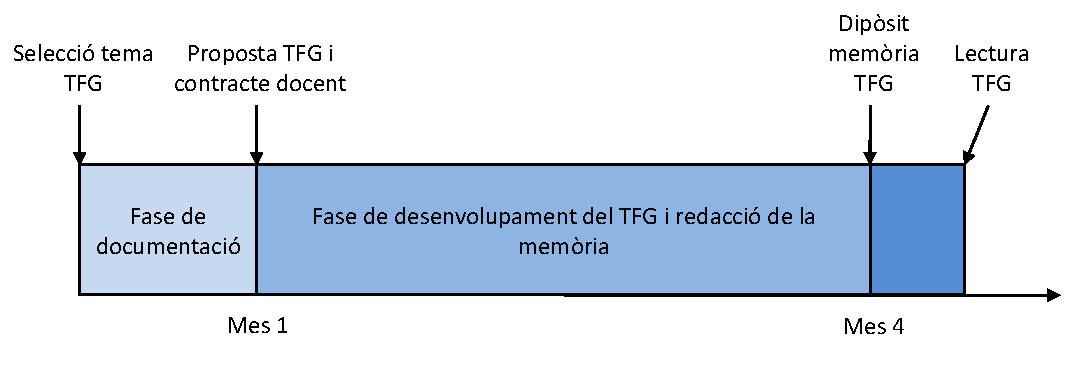
\includegraphics[width=\linewidth]{Itinerari_TFG}
% \caption{\label{fig:itinerari}Itinerari del Treball Final de Grau}
% \end{figure}

\section{Matrícula del Treball Final de Grau}

Com a norma general, tal com apareix reflectit en els plans d'estudis de gairebé totes les titulacions de grau, el \ac{TFG} s'hauria de realitzar en el quart curs. Tanmateix, tot i que aquestes s'agrupen en cursos i semestres, els estudis universitaris s'estructuren en assignatures. La normativa de l'\acf{EPS} marca que per tal de poder-se matricular al \ac{TFG} l'estudiant ha d'haver superat, o estar matriculat, de totes les assignatures del pla d'estudis, llevat de (com a màxim) 18 ECTS optatius.

\section{Selecció del tema de Treball Final de Grau}

La via estàndard per escollir el tema de \ac{TFG} és a través de l'eina dedicada a la gestió dels \ac{TFG}, accessible des de la web  de l'\ac{EPS}. En aquest cas, després de revisar les propostes realitzades pels diferents professors involucrats en la docència de l'\ac{EPS}, escollirem la que més ens interessi i, a través de la mateix eina web, farem la sol·licitud corresponent. Aquesta sol·licitud serà revisada pel professor responsable de la proposta i, si aquesta és acceptada, ens assignarà el tema de \ac{TFG} i s'iniciarà el procés de realització del TFG.

Existeixen altres possibilitats a l'hora d'escollir un tema de \ac{TFG}. Per exemple, podem realitzar el \ac{TFG} en una empresa del sector. En aquest cas és important que contactem amb un professor de l'\ac{EPS} que vulgui realitzar les tasques de tutorització i que pertanyi a un àrea de coneixement propera als continguts a tractar en el \ac{TFG}, d'aquesta manera ens assegurarem que la proposta de \ac{TFG} i el camp que aquesta cobreix compleixen amb els estàndards habituals a la nostra titulació. A més, caldrà designar un supervisor de l'empresa que faci el seguiment del treball i coordini amb el tutor acadèmic. En cas de dubte, el més convenient és contactar amb el cap d'estudis de la titulació corresponent que segur que ens orientarà i ens proporcionarà la informació necessària.

Val a dir que el \ac{TFG} també es pot realitzar en una universitat amb la que s'hagin establert convenis de convalidació (programes Sèneca, Erasmus, Averroes, \ldots). Tanmateix, en aquest cas haurem de seguir els procediments administratius establerts en aquesta altra universitat.

% \section{Preparació de la proposta i contracte docent}

% Un cop escollit el tema de \ac{TFG} començarem a treballar en la fase de documentació i, d'acord amb el nostre supervisor, prepararem la proposta de \ac{TFG}. Per a la redacció d'aquesta proposta convé seguir les indicacions descrites al capítol \ref{proposta} i és recomanable que aquesta fase de documentació i preparació de la proposta de \ac{TFG}, tal com es mostra a la Fig. \ref{fig:itinerari}, no s'allargui més enllà d'un mes. Sobre la proposta de \ac{TFG} és sobre la que estudiant i professor signaran el contracte docent. En aquest contracte s'establiran els compromisos del professor quant a seguiment i supervisió del projecte i els de l'estudiant quant a dedicació i termini de presentació. La proposta de \ac{TFG} i el contracte docent, signat tant per l'alumne com pel professor, seran lliurats als serveis administratius on l'\ac{EPS} signarà el compromís de disponibilitat de medis materials genèrics i de formalització d'un tribunal de \ac{TFG} adient.

\section{Desenvolupament del Treball Final de Grau}

Un cop aprovada la sol·licitud de \ac{TFG} per part del tutor, ens dedicarem a la realització del \ac{TFG} i a la redacció de la memòria sota la supervisió del tutor i amb els recursos disponibles que s'han posat a la nostra disposició segons la informació donada en la proposta de \ac{TFG}. Per a la redacció de la memòria convé seguir les indicacions descrites al capítol \ref{memoria}. 

\section{Dipòsit de la memòria}

Una vegada acabada la seva redacció, i amb el vist-i-plau del nostre supervisor, dipositarem la memòria del \ac{TFG} a secretaria seguint les indicacions de la normativa de \acsp{TFG} de l'\ac{EPS}. Cal tenir en compte que el tutor haurà de validar la documentació dipositada per l'estudiant, i que en cas de no estar conforme amb alguna part de la memòria o altre documentació lliurada, podrà retornar-la a l'estudiant per tal que aquesta sigui revisada i corregida. 

De manera excepcional, el tutor podrà autoritzar la tramitació del dipòsit tot deixant constància expressa de la seva disconformitat amb el treball presentat, i que la tramitació es fa sota la responsabilitat exclusiva de l’estudiant. 

Un cop acceptada la tramitació, aquesta serà revisada pel tribunal de \ac{TFG} que s'hagi assignat al nostre treball. Si el tribunal considera que la memòria no compleix amb els requisits mínims, podrà retornar-la a l'estudiant per tal que aquesta sigui revisada i corregida. 



\section{Preparació de la presentació}

Finalment només ens quedarà preparar la presentació del \ac{TFG} per tal de fer-ne la defensa oral davant el tribunal. Per a la preparació d'aquesta presentació convé seguir les indicacions del capítol \ref{presentació}.
